\addtocounter{section}{1}

\section{Préparation}

\begin{flushleft}
    Au cours de cette préparation, nous allons concevoir deux filtres passifs (composées d'inductances et capacités). Le but est d'utiliser les coefficients normalisés $g_i$ vu en cours pour modéliser les deux filtres théoriques afin de les comparer à la réalité.
\end{flushleft}
\subsection{Filtre 1 - Passe-bas de Chebyshev}
\begin{itemize}
    \subsubsection{Spécifications}

    \begin{flushleft}
        Le premier filtre passif à concevoir est un filtre passe-bas de Chebyshev d'ordre 6, de fréquence de coupure $f_c=11.1MHz$ et d'une ondulation de 0.2dB dans la bande passante pour impédance de normalisation $R_0=140${\Omega}.
    \end{flushleft}
    
    \subsubsection{Gabarit}
    \begin{figure}[!htbp]
      \centering
      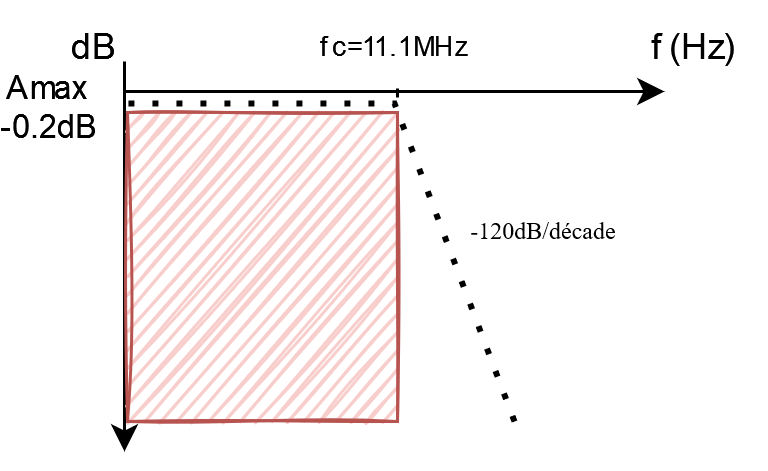
\includegraphics[scale=0.40]{img/passe_bas.png}
      \caption{Gabarit filtre passe-bas 6ème ordre Chebyshev}
      \label{fig:boat1}
    \end{figure}
    \FloatBarrier

    \subsubsection{Conception du filtre}
        \begin{flushleft}
            Une fois le gabarit du filtre réalisé, nous pouvons réaliser le schéma électrique du montage à partir du cahier des charges.
            La configuration est de type B, c'est-à-dire le premier élément du filtre passe-bas prototype est de type inductif.
        \end{flushleft}
        
        \begin{figure}[!htbp]
        \subfile{circuits/circuit_passe_bas} 
        \end{figure}
        \FloatBarrier
        
        \begin{flushleft}
            Pour déterminer les valeurs théoriques des inductances et capacités, on doit se réferer à la table des coefficients normalisés $g_i$, ou utiliser un programme Python destiné au calcul automatique de ces coefficients, celui-ci est disponible sur le notebook Jupyter de l'UGA.
        \end{flushleft}
        \newpage
        
        \begin{figure}[!htbp]
        \begin{mintedbox}{python}
n=6
delta = 0.2
fc = 11.1e6
omega_c = 2*π*fc
R0 = 140
g = chebyCoeff(delta, n)
#type B, on commence par une bobine
print("R0=", R0, 'Ohm')
for i in range(1,n+1) :
    
    if (i % 2) == 1 : # impair, L
        print("  L"+str(i)+"=", R0*g[i]/omega_c*1e6, "microH")
    else :
        print("  C"+str(i)+"=", g[i]/(R0*omega_c)*1e12, "pF")
print("R"+str(n+1)+"=", g[n+1]*R0, 'Ohm')\end{mintedbox}
        \caption{Programme Python pour calculs des valeurs des composants (Source: Sébatien Soulan, Notebook UGA)}
        \end{figure}
        \FloatBarrier
        
        \begin{figure}[!htbp]
        \begin{mintedbox}{python}
R0= 140 Omh
  L1= 2.729632808443258 microH
  C2= 139.61582010328723 pF
  L3= 4.49541437465984 microH
  C4= 149.0737852491278 pF
  L5= 4.210203447731343 microH
  C6= 90.51817278260027 pF
R7= 215.39737937478571 Omh\end{mintedbox}
        \caption{Valeurs retournées pour le filtre passe-bas Chebyshev ordre 6}
        \end{figure}
        \FloatBarrier
        \begin{flushleft}
            Il est important de remarquer que ces valeurs de capacités et d'inductances sont purement théoriques, il ne sera pas possible dans la réalité d'avoir ces valeurs exactes.
        \end{flushleft}
\end{itemize}

\subsection{Filtre 2 - Passe-bande de Chebyshev}
\begin{itemize}
    \subsubsection{Spécifications}
        \begin{flushleft}
            Le second filtre passif à concevoir est un filtre passe-bande de Chebyshev d'ordre 8, de fréquence de centrale $f_0=15.7MHz$, de bande passante relative $\frac{\Delta f}{f_0} = 0.3$ et d'une ondulation de 0.1dB dans la bande passante pour une impédance de normalisation $R_0=125${\Omega}.
        \end{flushleft}
    \subsubsection{Gabarits}
    \begin{flushleft}
        La méthode est de transformer un filtre passe-bas en passe haut via la forume suivante:
        $j.\omega \rightarrow Q.(j.\omega+\frac{1}{j. \omega})$
    \end{flushleft}
    
    \begin{figure}[!htbp]
      \centering
      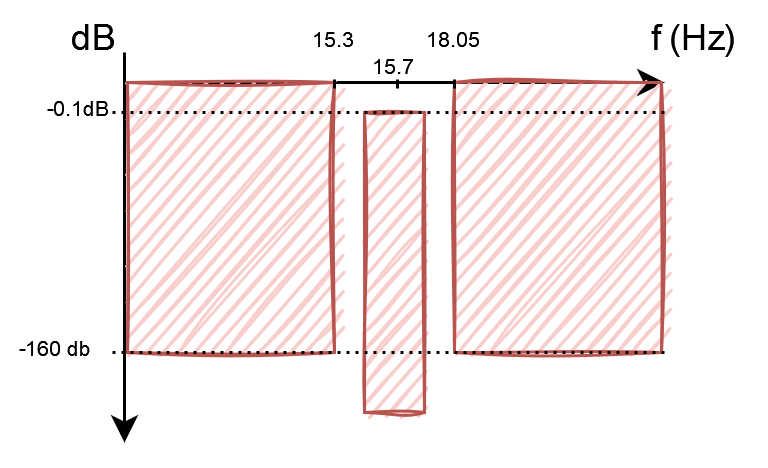
\includegraphics[scale=0.40]{img/passe_bande_simplifie.png}
      \caption{Gabarit simplifié filtre passe-bande 8ème ordre Chebyshev}
      \label{fig:boat1}
    \end{figure}
    \FloatBarrier
    \begin{figure}[!htbp]
      \centering
      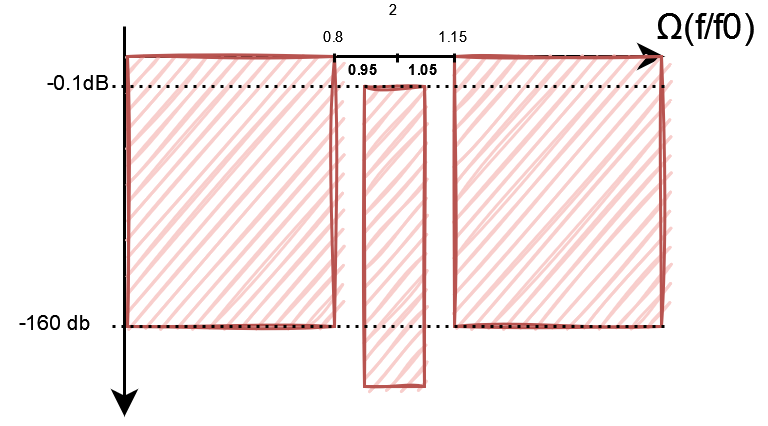
\includegraphics[scale=0.40]{img/passe_bande_normalise.png}
      \caption{Gabarit normalisé filtre passe-bande 8ème ordre Chebyshev}
      \label{fig:boat1}
    \end{figure}
    \FloatBarrier
    \begin{figure}[!htbp]
      \centering
      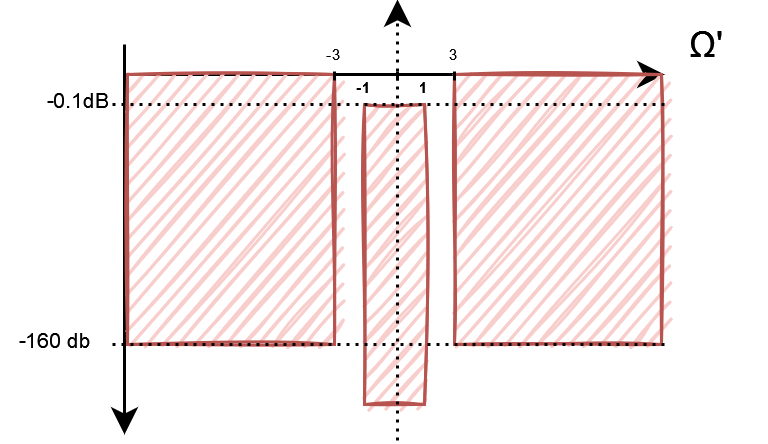
\includegraphics[scale=0.40]{img/passe_bande_prototype.png}
      \caption{Gabarit prototype filtre passe-bande 8ème ordre Chebyshev}
      \label{fig:boat1}
    \end{figure}
    \FloatBarrier
    
    \newpage
    \subsubsection{Conception du filtre}
    
    \begin{flushleft}
        Le but, est de faire une transformation de filtre passe-bas en filtre passe-bande. Les condensateurs en parallèle devienent des condensateurs et inductances en parallèle.
        Les inductances en séries deviennent des inductances et capacités en série.
    \end{flushleft}
    
    \begin{flushleft}
        Une fois les gabarits du filtre réalisés, nous pouvons réaliser le schéma électrique du montage à partir du cahier des charges.
    \end{flushleft}
    
    \begin{figure}[!htbp]
        \subfile{circuits/circuit_passe_bande} 
    \end{figure}
    \FloatBarrier
    
    \begin{flushleft}
        En utilisant les formules, nous pouvons déduire les valeurs des capacités et inductances pour le filtre passe-bande:
        $$ \frac{L_i.\omega_{0}}{R_0} = \frac{1}{R0.C_i.\omega_0}$$
        $$ Q = \frac{\omega_0}{\omega_{ch}-\omega{cb}}$$
    \end{flushleft}
    \begin{flushleft}
        On décide de calculer les valeurs des composants à partir du script python du Notebook.
    \end{flushleft}
    
    \begin{figure}[!htbp]
        \begin{mintedbox}{python}
n=4
delta = 0.1
fc = 15.7e6
omega_c = 2*π*fc
R0 = 125
Q = 1/0.3
g = chebyCoeff(delta, n)
#type B, on commence par une bobine
print("R0=", R0, 'Omh')
for i in range(1,n+1) :
    if i % 2 == 1 : # impair, L
        print("  L"+str(i)+"=", (R0*g[i]*Q/omega_c)*1e6, "microH")
        print("  C"+str(i)+"=", (1/(R0*g[i]*Q*omega_c))*1e12, "pF")
    else :
        print("  L"+str(i)+"=", (R0/(g[i]*Q*omega_c))*1e6, "microH")
        print("  C"+str(i)+"=", (g[i]*Q)/(R0*omega_c)*1e12, "pF")
        print("R"+str(n+1)+"=", g[n+1]*R0, 'Omh')\end{mintedbox}
        \caption{Programme Python pour calculs des valeurs des composants (Source: Sébatien Soulan, Notebook UGA)}
    \end{figure}
        \FloatBarrier
    \begin{figure}[!htbp]
        \begin{mintedbox}{python}
R0= 125 Omh
  L1= 4.683359227664407 microH
  C1= 21.94236766118584 pF
  L2= 0.29103648864763393 microH
  C2= 353.0965843504215 pF
  L3= 7.477710334435221 microH
  C3= 13.742708057249368 pF
  L4= 0.4646849522033069 microH
  C4= 221.14766052906083 pF
R5= 169.42016809801058 Omh\end{mintedbox}
        \caption{Valeurs retournées pour le filtre passe-bande Chebyshev ordre 8}
        \end{figure}
        \FloatBarrier
\end{itemize}

\subsection{Filtre 3 - Passe-bas elliptique}
\begin{itemize}
    \subsubsection{Spécifications}
        \begin{flushleft}
            Le dernier filtre que nous allons études est un filtre passe-bas elliptique d'ordre 4, de fréquence de coupure $f_c=4.1MHz$, d'une ondulation de 1dB dans la bande passante et 52dB d'affaiblissement minimum en bande coupée 10MHz.
        \end{flushleft}
    \newpage
    \subsubsection{Gabarit}
    \begin{figure}[!htbp]
      \centering
      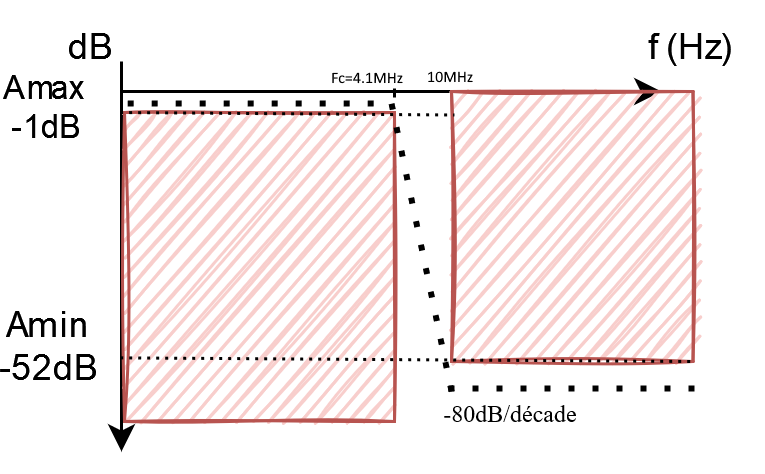
\includegraphics[scale=0.40]{img/elliptique.png}
      \caption{Gabarit simplifié filtre passe-bas 4ème ordre Elliptique}
      \label{fig:boat1}
    \end{figure}
    \FloatBarrier
    
\end{itemize}

\newpage






